\section{Lecture 12: Sampling followed by Linear Interpolation}


\subsection{Introduction}
In the previous section, we have seen the working of a Sample and Hold circuit. We can now say that the Sample and hold circuit is nothing but an Ideal Sampling System followed by a Linear Shift Invariant system.

We have also seen the drawbacks of the sample and hold circuit which include:

\begin{enumerate}
\item Distortion in the original spectrum.
\item Aliases also pass through the circuit partially.
\end{enumerate}

We will now look at the procedure that will be followed by the Sample and Hold circuit.
\subsection{Linear Interpolation}
Linear Interpolation can be broadly defined as the joining of two known points by a straight line.

Thus, if we know two given points, the linear interpolant will be the straight line joining these two lines. 

\begin{figure}[h]
\centering
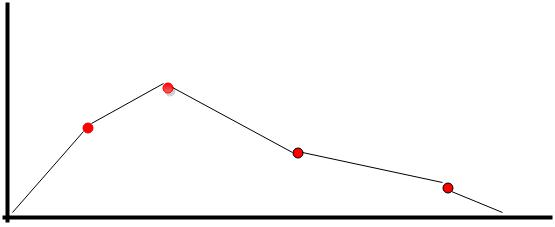
\includegraphics[width=0.9\linewidth, height=4cm]{LinInt.jpg}
\caption{Linear Interpolation of given points.}
\end{figure}
\label{sec:examples}

Above figure indicates a rough sketch of Linear Interpolation of a given set of points. 



\pagebreak

\subsection{Signal Representation of Linear Interpolation}

We now look at the effect of the Linear Interpolation on a given signal $x(t)$.

Signal $x(t)$ is passed through an ideal sampler, with sampling interval $Ts$.

It is then passed through a Linear Shift Invariant system.

\begin{figure}[h]
\centering
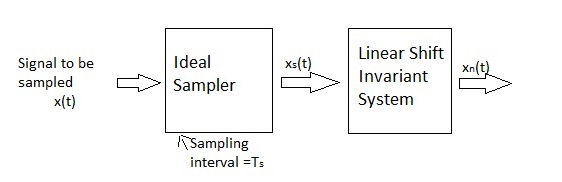
\includegraphics[width=0.7\linewidth, height=3cm]{M3L12-fig4.jpg}
\caption{Passing x(t) through the Sample and Hold Circuit.}
\end{figure}
\label{sec:example}
\paragraph{}
\paragraph{}
The impulse response of the Linear Shift Invariance will be triangular in nature as shown below. 
We sketch the original signal $x(t)$, the ideal sampling output $xs(t)$ and the scaled and shifted impulse response of the Linear Shift Invariant System given by $x(nTs).h(t-nTs)$

\begin{figure}[h]
\centering
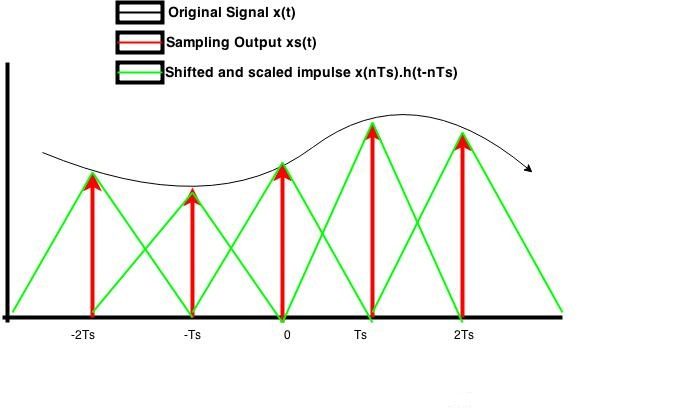
\includegraphics[width=0.9\linewidth, height=4cm]{graph1.jpg}
\caption{Signal Representation along with the Sampling output and the Impulse response of LSI system}
\end{figure}

\paragraph{}
\paragraph{}
The shifted and scaled impulse responses are now added linearly. As seen before, linear interpolation is the joining of two points with a straight line.

We now add the $green$ straight lines between the various time intervals. Additions of two straight lines will also be a straight line. 

The resulting addition of these straight lines will be the Linear Interpolated Signal and can be seen in $blue$ in the figure below.
\pagebreak

\begin{figure}[h]
\centering
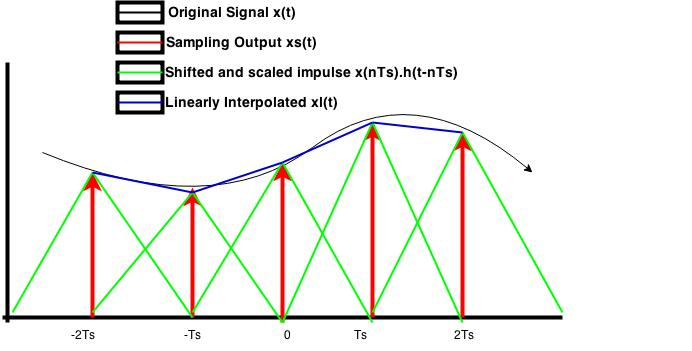
\includegraphics[width=0.9\linewidth, height=4cm]{graph2.jpg}
\caption{Signal Representation along with the Sampling output and the Impulse response of LSI system}
\end{figure}
\paragraph{}
Idea of Linear Interpolation for a signal can be stated as the passing of an ideally sampled output through a Linear Shift Invariant system.
\paragraph{}
\paragraph{}
\subsection{Significance in frequency domain}

Convolution of a signal with itself can be seen as the multiplication of it's Fourier Transform with itself. 

The sample signal $h0(t)$ can be shifted to the time interval $-Ts/2$ to $Ts/2$.This gives us the Zero order hold. 

Convolution $h0(t)$ with itself gives us the first order hold. It can be seen in the given diagram.
\begin{figure}[h]
\centering
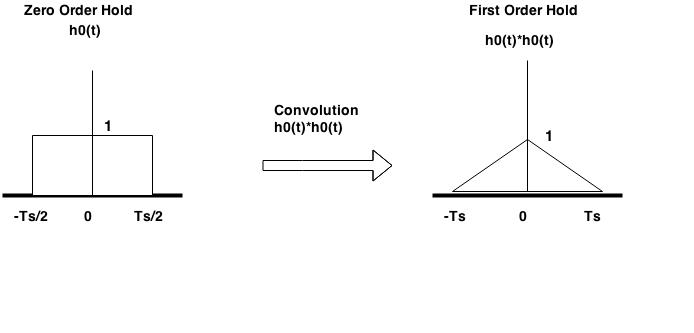
\includegraphics[width=0.9\linewidth, height=4cm]{graph3.jpg}
\caption{Convoluting the Zero order hold with itself}
\end{figure}
\pagebreak

\subsubsection{Mathematical representation}

Frequency Response of first order hold:
$$Ts.\exp(-jt\omega).\frac{sin(\frac{Ts}{2}\omega)}{\frac{Ts}{2}\omega}.\exp(\frac{Ts}{2}\omega)$$

Squaring the above term, we get:

$$Ts^2.(\frac{sin(\frac{Ts}{2}\omega)}{\frac{Ts}{2}\omega})^2$$

The implications will be as follows:
\begin{enumerate}
\item sinc(fTs) has a maximum value of 1.
\item We know that the function $sinc(fTs)$<1. Therefore, squaring the function will result in further reduction of magnitude.
\item The function will thus fall at a faster rate.
\end{enumerate}

We can thus conclude from above that the given operation has the following effects on the signal band:

\begin{description}
\item[Advantages] We can thus see that the side lobes are now lower. The other aliases that were formed are suppressed as compared to the Zero order hold.

\item[Disadvantage] Along with the side lobes, the major lobe too will now be suppressed to some extent. The region from $-Ts/2$ to $Ts/2$ suffers a steeper drop.  
\end{description}






